%\documentclass[11pt]{article}
%\usepackage{fullpage}
%\usepackage{graphicx}
%\usepackage{indentfirst}
%\usepackage[font=small, labelfont=bf, skip=1pt]{caption}

%\begin{document}

\subsection{External interface requirements}
\subsubsection{User interfaces}
The following mockups represent a basic idea of what the mobile app will look like in the first release. The last one shows instead an idea about the minimal interface of the wearable application. \newline

\begin{figure}[h!]
\centering
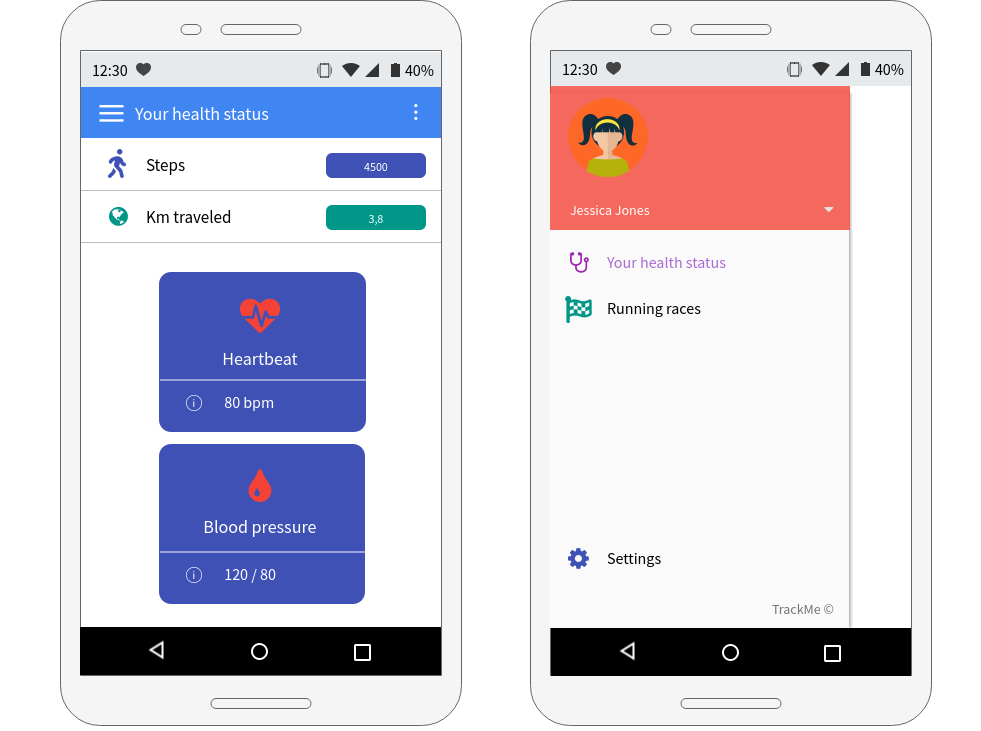
\includegraphics[scale=0.45]{sections/mockups/mockups1,2.png} \newline
\captionof{figure}{[Mockup] - Home page of user's account (the user can monitor his/her own parameters)}	\captionof{figure}{[Mockup] - Side menu \newline}	
\end{figure}

\clearpage

\begin{figure}[h!] \ContinuedFloat
\centering
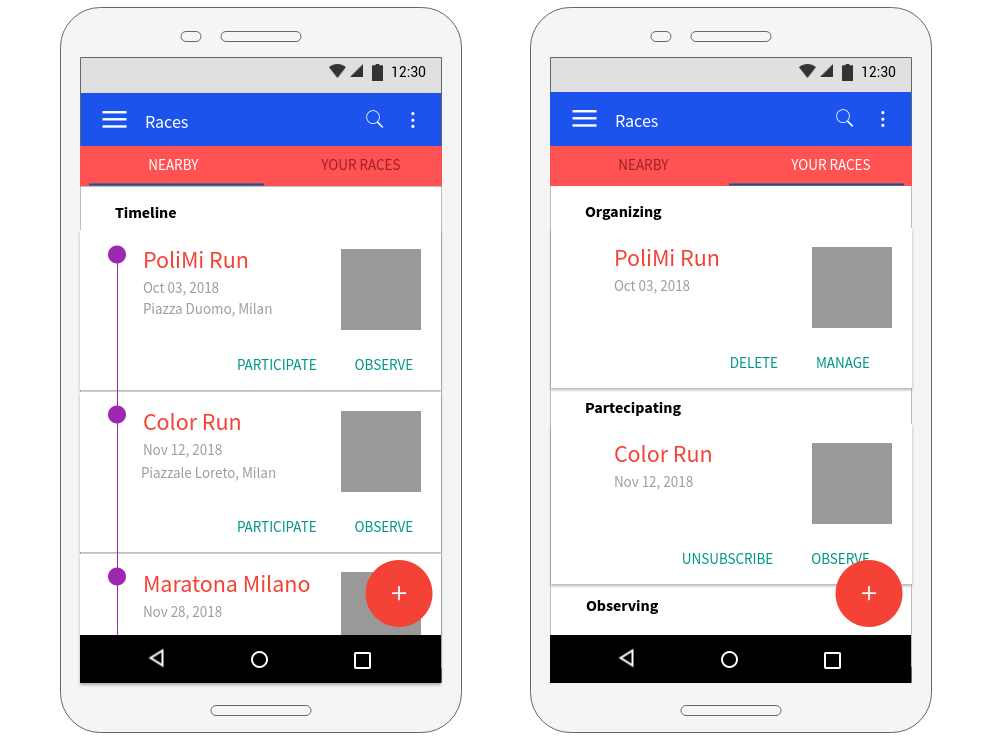
\includegraphics[scale=0.45]{sections/mockups/mockups3,4.png} \newline
\captionof{figure}{[Mockup] - Races screen (NEARBY tab)}
\captionof{figure}{[Mockup] - Races screen (YOUR RACES tab)}
\end{figure}

\begin{figure}[h!] \ContinuedFloat
\centering
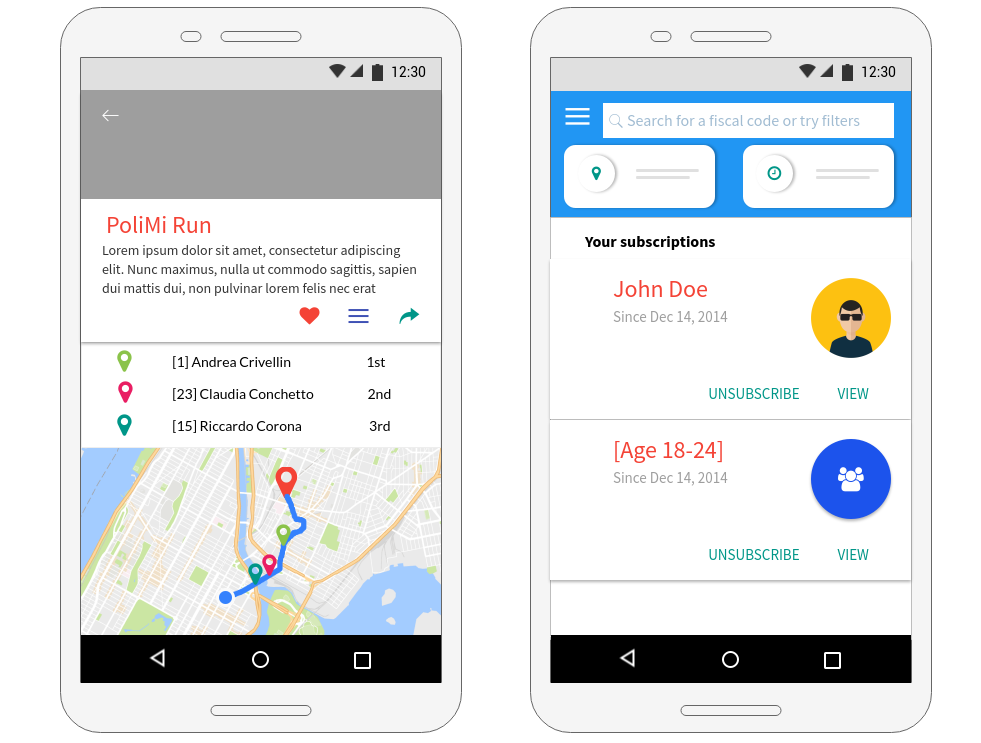
\includegraphics[scale=0.45]{sections/mockups/mockups5,6.png} \newline
\captionof{figure}{[Mockup] - Race overview with leaderboard and track}
\captionof{figure}{[Mockup] - Home page of company's account (the company can search and manage data)}
\end{figure}

\clearpage
	
\begin{figure}[h!] \ContinuedFloat
\centering
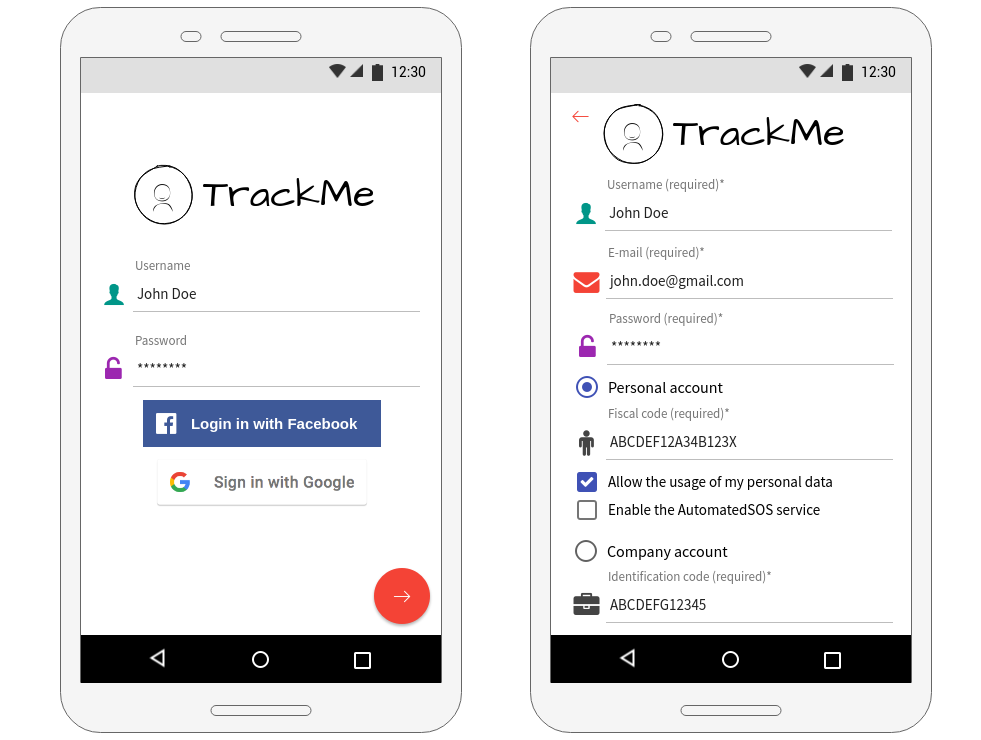
\includegraphics[scale=0.45]{sections/mockups/mockups7,8.png} \newline
\captionof{figure}{[Mockup] - Login screen}
\captionof{figure}{[Mockup] - Registration screen}
\end{figure}
	
\begin{figure}[h!] \ContinuedFloat
\centering
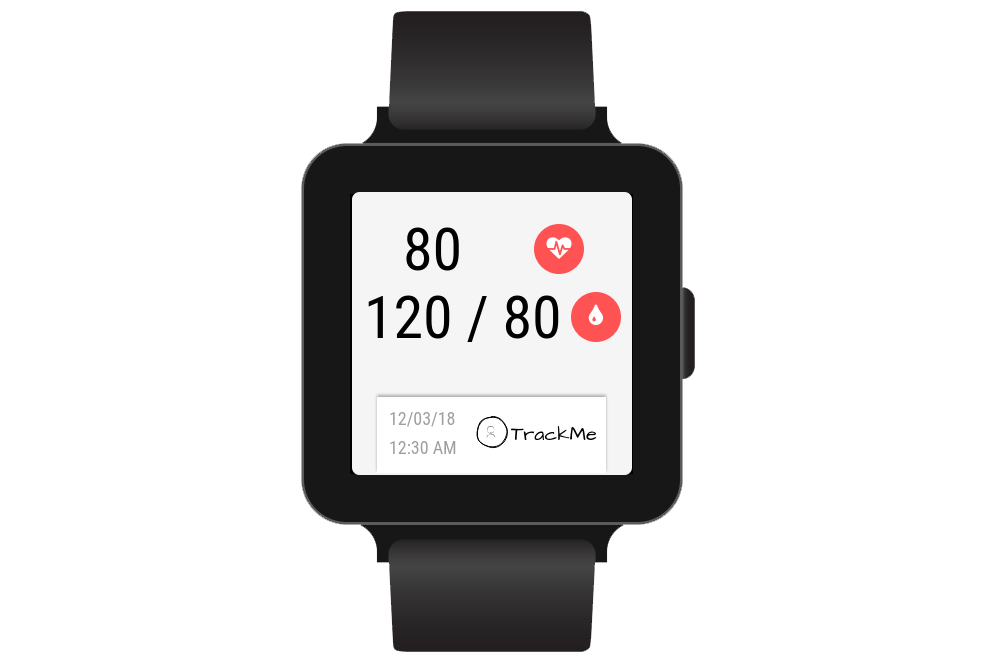
\includegraphics[scale=0.45]{sections/mockups/mockupWatch.png} \newline
\captionof{figure}{[Mockup] - Example of the app screen on a smartwatch}
\end{figure}

\subsubsection{Hardware interfaces}
The application doesn't use any hardware interface, however a smartphone paired with a wearable device like a smartwatch or a fitness tracker is required to use the Data4Help and AutomatedSOS services, and to participate to races using Track4Run (pairing in most cases is made via bluetooth).

The wearable device must have at least the following sensors: GPS, accelerometer, altimeter, gyroscope, heart rate sensor. Blood pressure sensor is also supported by the app and devices equipped with it are highly recommended for a complete experience with TrackMe.

Organizers and spectators of running races, and also third parties can manage their activities without specific hardware requirements (wearable device not required for their tasks).

Users who own a smartwatch with Wear OS can also download a TrackMe version specifically designed for this kind of devices.

\subsubsection{Software interfaces}
\subsubsection{Communication interface}

\subsection{Scenarios}
\subsubsection{Scenario 1}
Aurora is a non-profit organization that deals with disabled young people. Aurora's board of directors decided to use TrackMe to support medicians in their work and monitor the health status of patients in a more efficient way. Most of the patients, according with their parents, decided to download the app on their smartphone. Aurora's medicians were able to estimate the average course of the heartbeat and blood pressure of patients just searching for anonymous data using the age filter (18-21 years old) and the location filter (via Aurora 2, Perugia) and subscribing to the search results.

\subsubsection{Scenario 2}
Davide is the athletic trainer for the under 21 athletes of Milano Atletica. He decided to organize a competition between his student, so he launched TrackMe and created a new running race in the "Your running races" section, using the "+" button. He selected the location of the sport center (via Cimabue, Milan) and established the date of the race (15/11/2018) and the closing date of the registrations (14/11/2018). He obviously decided to select the partecipants sending them invites to join the competition.

Giovanni, one of his students, immediately joined the competition but unluckily he was not able to compete due to an injury. Through the "MANAGE" option Davide was able to mark him as "disqualified" in order to effectively know the participants in the race and monitor their performances.

\subsubsection{Scenario 3}
Lidia is an elderly woman who loves walking. His grandson Matteo suggested her to download the TrackMe app on her smartphone paired with her fitness tracker, in order to monitor her own activities and health status and also to make sure his grandmother receives assistance in case of health problems.

One day, during a walk, Lidia felt sick and collapsed on the ground. TrackMe detected an abnormality in the heartbeat and called immediately the 112, sending also an SMS with her position, heart rate and blood pressure. The ambulance intervened a few minutes later and Lidia was successfully rescued.

\subsection{Functional Requirements}
\hspace{-\parindent}\textbf{[G1] - Users and third parties can be recognized by providing a form with their data} \newline

[R1] -  The usernames used in the system are unique to every user and third party. \newline

[D1] - Third parties own an alphanumerical code received from a TrackMe administrator used to verify their identities and match them with the company account. \newline

[R2] - Users and third parties can create an account by compiling a form. \newline

\hspace{\parindent}[R2.1] - The form should contain the following: username, password, choice between user and third party account, other anagraphical info (for the user) or company info (for the third party). \newline

[R3] - Third parties must provide an identification alphanumerical code to confirm their identity. \newline

[R4] - Users and third parties can log in to the application by providing the combination of a username and a password that match an account. \newline

\hspace{-\parindent}\textbf{[G2] - Allow third parties to access to the data of some specific individuals} \newline

[D2] - Device sensors can provide accurate data to the app. \newline

[R5] - Third parties can search for specified data by filling the search bar with the fiscal code of a specific user. \newline

[R6] - A notify is sent to the selected user, who can accept or refuse the sharing of data with the specific company. \newline

[R7] - A message is sent to the third party, containing user's data if he/she allowed the sharing or a notification of refuse otherwise. \newline

[R8] - Users under 18 years old can't be shown in the results of a search. \newline

\hspace{-\parindent}\textbf{[G3] - Allow third parties to access to anonymized data of groups of individuals} \newline

[R9] - Third parties can search for anonymized data of a specific group of users by selecting search filters (location, age, sex, time slot). \newline

[R10] - Anonymized data are shown just if the research produces at least 1000 results. \newline

\hspace{-\parindent}\textbf{[G4] - Allow third parties to subscribe to new data and to receive them as soon as they are produced} \newline

[R11] - Third parties can flag an option to subscribe to new data of a specific user when they receive his/her data (the user already allowed the data sharing), or they can subscribe to get results of a research with specific filters as soon as they are produced. \newline

[R12] - Third parties can manage their subscriptions in a management section in the app. \newline

\hspace{-\parindent}\textbf{[G5] - Allow the users, through the AutomatedSOS service, to come help by an ambulance when such parameters fall below certain thresholds} \newline

[D3] - TrackMe is affiliated with NUE 112 (Numero Unico per le Emergenze) to offer assistance in Europe, and with 911 to offer assistance in the USA. \newline

[R13] - Users can manage the subscription to the AutomatedSOS service through a specific option in the settings menu. \newline

[R14] - Old users (60+ years old) are automatically subscribed to the AutomatedSOS service since their registration. \newline

[R15] - The app calls autonomously the NUE (or 911) when such parameters fall below certain thresholds, and sends concurrently user's data (GPS location and health status parameters) via SMS. \newline

\hspace{-\parindent}\textbf{[G6] - Allow racing organizers, through the Track4Run service, to manage runs and define a path for runs} \newline

[R16] - Users can create races by defining name, date, time, start point, stages and arrival point, and selecting the method of partecipation (open or by invitation) and the date and time of expiration for registrations. \newline

\hspace{\parindent}[R16.1] - If a race by invitation is selected, a private link to a registration page is generated. \newline

[R17] - The system allows the organizers to sign an enrolled runner as "present" and to disqualify a runner by signing him/her as "disqualified". \newline

[R18] - Users can manage their orga in a management section in the app. \newline

\hspace{\parindent}[R18.1] - Organizers can postpone or delete a run. A notification is sent to partecipants and spectators. \newline

\hspace{-\parindent}\textbf{[G7] - Allow racing partecipants to enroll runs} \newline

[R19] - Users can visualize nearby races or search for a specific run by searching for the name or location of the race. \newline

[D4] - The run can be joined only by persons enrolled through the app. \newline

[D5] - If it is required a payment to enroll a run, an external service will guarantee secure transactions and receipts by e-mail. \newline

[R20] - Runners can join a race through the race overview by clicking the "Participate" button. For races by invitation the button is visible just to invited users following the registration link. \newline

\hspace{\parindent}[R20.1] - If it's specified that some payment is required, it will be committed to an external service. \newline

[R21] - When the race starts, the partecipant have to wear his/her wearable device with Data4Help installed. \newline

\hspace{-\parindent}\textbf{[G8] - Allow racing spectators to see on a map the position of all runners during the run} \newline

[R22] - Users can become spectators of a race through the race overview by clicking the "Observe" button. \newline

[R23] - For the duration of the race is always possible to see in the event page the map with markers, associated to runners' name through numbers, and a live leaderboard showing names, order numbers and possible disqualifications. \newline

[R24] - A marker is on the track iff it corresponds to a user enrolled, signed as "present" at the run with his/her wearable device with Data4Help installed and not disqualified. \newline

[R25] - The track represented is the one chosen by the organizer of the run. \newline

[R26] - Markers move according to the corresponding persons' movement, as reported by the location service. \newline

\hspace{-\parindent}\textbf{[G9] - Allow users to monitor their own health status} \newline

[R27] - Users can visualize their own health status in the home page section of the app. \newline

%\end{document}